\subsection{Review of the literature}

\begin{figure}[h]
\begin{center}
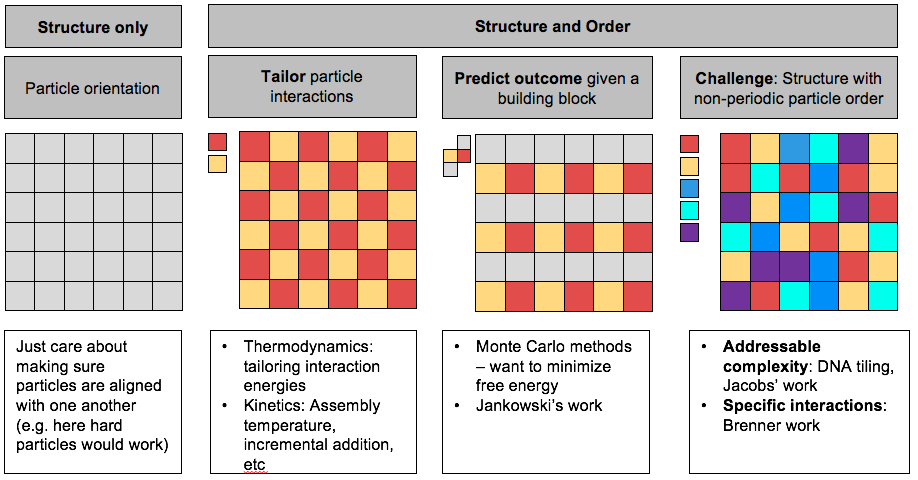
\includegraphics[width=6.5in]{../figures/litreview.png}
\caption{Demonstration of the state of the art in the literature}
\label{fig:litreview}
\end{center}
\end{figure}

Let's take a simple system and use it to illustrate the state of the art in the theory for engineering self-assembly behavior.

Let us say that we have the simple target 2D array shown in Figure \ref{fig:litreview}.

% =====
% STRUCTURE ONLY
% ====
If we assume all the particles in our system are uniform, we simply care about making sure particles assemble into the target structure.
As in any type of assembly, this implies a minimization of free energy.
In the example of hard squares above, minimization of free energy corresponds to a maximization of entropy.

\begin{itemize}
\item Archimedean tilings
\item Glotzer work on assembling target structures
\end{itemize}


\cite{vanAnders_2014_ACSNano}: Can treat shape as giving particles an effective entropic patchiness

\cite{Millan_2014_ACSNano}:
Develop a metric of self-assembly complexity, flow chart in Figure 3.
Archimedean tilings (ATs)
Here, we report the minimal set of interactions needed to self-assemble experimentally accessible ATs from regular polygons, mimicking nanoplates assembled into crystalline monolayers (Figure 1). We show through Monte Carlo simulations the self-assem- bly of these tilings by exploiting entropic and enthalpic interactions encoded in the shape of the polygons. We arrive at a design strategy for patchy polygon particles that is accessible to current experimental techniques and present the minimal set of design rules for each AT. We report that four ATs, namely, the (63), (36), (44), and (3.122) tilings, can be assembled solely with hard interactions, highlighting the role of directional entro- pic forces39,40 that arise from the particle shape.

After selecting the building blocks, the design pro- cess examined the constituent polygonal building blocks and alters the interaction complexity by chan- ging the specificity of interactions. The four models ranked in terms of specificity are hard, symmetric patches, shape-specific patches, and edge-specific patches

Manually adds complexity in the amount of specificity:
Initially, we test if entropic interactions are sufficient to self-assemble each crystalline structure. If the infinite pressure ground state (hard particle) won't assemble the target structure, add attractive interactions. If the crystalline structure for a mixture of building blocks does not contain the alternating building block property, it is necessary to use edge-specific interactions.


% =====
% STRUCTURE AND ORDER: TAILORING PARTICLE INTERACTIONS
% ====
As we look to make more complex materials, though, we also want to specifically order the particles within a structure.
We can approach this through tailoring the thermodynamics and/or the kinetics.

\begin{enumerate}
\item Glotzer, Kotov work on patchy particles for getting different arrays/structures
\item BUBBA work
\item DNA tilings, DNA-tailored assembly
\item need to find some other citations here?
\end{enumerate}

\begin{enumerate}
\item \cite{Damasceno_2012_Science,Ye_2013_NatChem,Zhang_2004_NanoLetters}
\item \cite{Jankowski_2009_JChemPhys,Jankowski_2011_JPhysChemB,Jankowski_2012_SoftMatter}
\item \cite{Mirkin_1996_Nature,Park_2008_Nature,OBrien_2016_JACS}
\end{enumerate}

\cite{Ye_2013_NatChem}: Despite the apparent simplicity in particle geometry, the combination of shape-induced entropic and edge-specific energetic effects directs the formation and stabilization of unconventional long-range ordered assemblies not attainable otherwise.

\cite{Park_2008_Nature}: can create crystals using DNA functionalization
\cite{OBrien_2016_JACS}: Colloidal crystallization can be pro- grammed using building blocks consisting of a nano- particle core and DNA bonds to form materials with controlled crystal symmetry, lattice parameters, stoichiometry, and dimensionality. Can tailor DNA length and shape to get different crystal structures

DNA programmable assembly. The sequence-specific binding property of DNA can be applied to direct the assembly behavior of colloidal particles at the nanoscale. This is a powerful strategy to control nanomaterial assembly because it allows tuning of the interparticle interaction in highly specific ways. For example, attaching DNA linkers with self-complementary sequences to particles directs them to maximize the number of nearest neighbors, resulting in fcc arrangement. On the other hand, particles with non-self-complementary linkers, which only allow A-B contacts, assemble into bcc or CsCl-type arrangement by maximizing the number of A-B contacts around the first coordination shell \cite{Park_2008_Nature}.This technique has recently been applied to anisotropic particles and opened possibilities to access diverse crystal structures in nanoscale by employing the DNA programmability as well as geometrical properties of the anisotropic shapes (25, 26).Despite its powerful potential, studies regarding the assemblies of DNA-coated anisotropic colloids have until recently (Sangmin's paper) been limited to simple crystal structures with small unit cells (27, 28). 

% =====
% STRUCTURE AND ORDER: PREDICTING ASSEMBLY
% ====
To test the interactions we've tailored above, we also need to be able to test the assembly properties of these building blocks.
We want to see what structure they will assemble into to minimize their free energy.
Our initial instinct would be to run these simulations to steady state or equilibrium.
However, systems with complex interactions such as these can get themselves caught in metastable free energy local minima that MC methods may not have large enough energy fluctuations to escape from.
This is where thermodynamics and kinetics really come to play together

\begin{itemize}
\item BUBBA work
\item Wales work (disconnectivity graphs) - more of the thermo
\item Kinetic pathway design - Frenkel, Jacobs
\item Connectivity graphs to show the order of assembly
\item Pathway assembly sampling
\item swear I read something earlier today about metastable/kinetic traps
\end{itemize}



% =====
% STRUCTURE AND ORDER: THE BIG CHALLENGE
% ====

Real-world:
\begin{itemize}
\item Protein assembly
\item Complex DNA tiling, assembly - Mirken, Winfree, Rutherford, check semisynbio sources
\end{itemize}


Theory perspective:
\begin{itemize}
\item Addressable complexity
\item Efficiency of specific interactions
\end{itemize}



% =====
% THEORETICAL CHALLENGES
% ====
\begin{itemize}
\item Getting partition functions-- hard to find all the possible states; folks are trying to tackle this with information-theoretic approaches
\item Related to the above, even in 2D assembling structures given this level of specificity is a drag, and is not a simple model system (interactions between all the different particles, kinetics of the assembly, etc)
\item Figure \ref{fig:semisynbio} summarizes these challenges nicely
\item Need to find a simpler system
\end{itemize}


% =====
% PROPOSED SYSTEM
% ====
Folding nets are a pretty well-defined system. We need a system with limited degrees of freedom to establish these concepts.
\begin{itemize}
\item Paul's paper (Glotzer)
\item Demaine folding paper, and any additional citations
\item Origami papers
\end{itemize}




If we didn't care about the ordering of the $A$ and $B$ particles on the lattice, we know that we could leave the particles as hard particles with only volume exclusion, and at proper densities the system would self-assemble into a square lattice to maximize entropy [CITE].
However, we care about the order of species within the lattice.
Our goal is to give the $A$ and $B$ particles some interaction that allows them to kinetically and thermodynamically reliably assemble that target structure.

Have specific interactions between the particles

with interaction energies $\epsilon_{AB}$, $\epsilon_{BA}$, $\epsilon_{AA}$, and $\epsilon_{BB}$
%(These particles were initially conceived by Troisi \textit{et al} \cite{Troisi_2005_JChemPhys} and used by Jankowski and Glotzer \cite{Jankowski_2009_JChemPhys} to explore energy minimization algorithms for patchy particles.)

\textbf{Information as a measure of the likelihood of a particular configuration being preferred.}
In 2015, a review article in \textit{Nature Physics} (which has since been cited 255 times) reviewed the state of the art on applying information theoretic entropy-- i.e. Shannon entropy-- as a way of understanding non-equilibrium thermodynamics \cite{Parrondo_2015_NaturePhysics}.
In this work, they investigate information entropy as a placeholder for non-equilibrium entropy production.
This entropy production gives an overall likelihood of a configuration (one which minimizes the non-equilibrium free energy of a system while maximizing the non-equilibrium entropy).
However, this method applies to the overall structure, or the overall likelihood of a structure being the preferred structure.

\textbf{``Addressable complexity'' seeks to engineer pathways for particular particles to reach their destination.}
Low free energies of a target structure, however, do not guarantee efficient assembly.
There are a number of ways addressing this problem in the literature.
One way of forcing systems into assembly is to design a free energy landscape that minimizes such meta-stable traps \cite{Wales_2017_JChemPhys}.
Competition between degenerate structures of equivalent potential energy was reported for clusters of six attractive spherical colloids, where symmetry breaking leads to higher rotational entropy of the less symmetric conformation, resulting in lower free energy \cite{Meng_2010_Science}.

Taken from \cite{Jacobs_2015_JChemPhys}: 
A well-known example of addressable complexity-- that is, specific binding-- can be found in ``one-pot'' DNA self-assembly of DNA tiles, which use the hybridization of complementary DNA sequences to construct complex structures consisting of hundreds of subunits from a single soup of monomers \cite{Ke_2012_Science} (5).
Simulation results have shown that such one-pot self-assembly can succeed with highly simplified model subunits that lack the molecular details of DNA tiles, suggesting that similar design strategies should be widely applicable \cite{Reinhardt_2014_PRL} (6).
In the work by Jacobs \textit{et al}, they had particles with designed interactions between one another.
They represented the target bonds by a graph, $G$.
However, this model is based on the assumption that ``designed interactions in the target structure are typically much stronger than any incidental associations between sub-units that should not be connected in the final assembly''.
This is a fine assumption for their proof of concept, but is not valid in real-world system.
As a concrete example, protein-folding is perhaps the most well-explored biological system that assembles due to specific interactions \cite{Dill_1993_CurrOpinStructBiol}.
However, one of the major challenges to solving the protein-folding problem are competing ``cross-talk'' interactions [CITATIONS NEEDED; chaperoned folding and assembly Chakrabarty 2017].

In later work, Jacobs et al addressed this oversight and accounted for incidental interactions in addition to designed interactions \cite{Jacobs_2015_PNAS}.


Low energies may not guarantee efficient assembly
compartmentalized, multi-stage assembly
grannemana and baserga 2004

Talk outline:
1. self-assembly kinetics can be rationally designed-- leverage thermodynamics
2. evolution has already selected for optimal assembly pathways in complex biomolecules


\textbf{Specific binding interactions can be tailored to lead to target structures}.
However, there is a delicate balance of specificity required.
On the over-specified side, we have bonds that are specific to their intended neighbor with probability 1.0.
On the under-specified side, we have non-specific interaction patches that will bond to any other patch with probability $1/n$, where $n$ is the total number of patches in the system.

In work from our group, Eric Jankowski sought to generate energy-minimizing configurations for such patchy particles \cite{Jankowski_2009_JChemPhys} in a process he called ``bottom-up building block analysis'', or BUBBA.
Cluster Monto Carlo (cMC) and LAcMC methods are relatively poor methods for finding potential energy minima formed from patchy particles with disparate interaction energies due to their tendency to become trapped in metastable configurations as well as the low degeneracy of potential energy-minimizing configurations (Q).
BUBBA effectively searches a subset of the configuration space for energy-minimizing configurations.
Jankowski predicted that that BUBBA would be useful for evaluating many different particles for self-assembly ``propensity''.

Partition functions encode all the thermodynamics of a system, but for most systems of practical importance they cannot cannot be calculated exactly.
This is due to many indistinguishable degenerate states. 
In the cases where small numbers of distinguishable configurations comprise a majority of a partition functions' weight, as is the case for systems at low temperatures and for many anisotropic building blocks with disparate interactions, BUBBA is a particulalry effective method for generating partition functions that have been heretofore inaccessible. 
This allows us to ask ``What structures are thermodynamically favored for this building block at any temperature?'' to be answered independently of assembly kinetics. \cite{Jankowski_2011_JPhysChemB}

% Note: Jankowski_2011_JPhysChem has a really good introduction

Both thermodynamic and kinetic barriers to assembling target structures.

Key problem, taken from \cite{Jankowski_2012_SoftMatter}:
Self-assembly holds promise for creating new materials and devices because of its inherent parallelism, allowing many building blocks to simultaneously organize using preprogrammed interactions.
An important trend in nanoparticle and colloid science is the synthesis of particles with unusual shapes and/or directional (??patchy??) interactions, whose anisotropy allows, in principle, assemblies of unprecedented complexity.
However, patchy particles are more prone to long relaxation times during thermodynamically driven assembly, and there is no a priori way of predicting which particles might be good assembly candidates. 
Here we demonstrate a new conceptual approach to predict this information using sequences of intermediate clusters that appear during assembly.
\textbf{Unfortunately, when an equilibrium solution or simulation of patchy particles fails to generate an ordered pattern it is not always obvious whether the culprit is thermodynamics or kinetics.}
Recently there have been studies that attempt to quantify kinetic trapping through fluctuation-dissipation ratios (21,22) and through the interplay between specific and nonspecific interactions (3,5,23) but these methods do not provide predictive capabilities for thermodynamically stable structures.
The fact that both thermodynamics and kinetics can prevent a system of particles from self-assembling is particularly trou- blesome for experimentalists that search parameter space via trial-and-error because experiments that fail to assemble do not provide information about how assembly might be improved.


We are ultimately searching for rational design of building blocks optimized for self-assembly that focuses on assembly pathway engineering: identifying the traps that occur as a system assembles so they may be circumvented.
As systems self-assemble we hypothesize that the thermodynamically stable intermediate clusters that arise hold information about their ability to order. 
These sequences of intermediate clusters are assembly pathways and we propose a methodical analysis of them to predict the degree to which a system of building blocks will assemble a target pattern, which we refer to as the building block?s assembly propensity for the pattern.
We foresee assembly pathway engineering proceeding as a collaboration among structural identification, kinetic measurements, and the assembly pathway analysis described here. \cite{Jankowski_2012_SoftMatter}

\subsection{Motivation 1: DNA assembly, DNA tiles, DNA cubes}

Taken from intro of \cite{Reinhardt_2014_PRL}: \\
The observation by Ke et al. [Science 338, 1177 (2012)] that large numbers of short, predesigned
DNA strands can assemble into three-dimensional target structures came as a great surprise, as no colloidal
self-assembling system has ever achieved the same degree of complexity. That failure seemed easy to
rationalize: the larger the number of distinct building blocks, the higher the expected error rate for
self-assembly. The experiments of Ke et al. have disproved this argument. Here, we report Monte Carlo
simulations of the self-assembly of a DNA brick cube, comprising approximately 1000 types of DNA
strand, using a simple model. We model the DNA strands as lattice tetrahedra with attractive patches, the
interaction strengths of which are computed using a standard thermodynamic model. We find that, within a
narrow temperature window, the target structure assembles with high probability. Our simulations suggest
that misassembly is disfavored because of a slow nucleation step. As our model incorporates no aspect of
DNA other than its binding properties, these simulations suggest that, with proper design of the building
blocks, other systems, such as colloids, may also assemble into truly complex structures.

Need to include Winfree, Rutherford papers in here.

Include work from NSF proposal.

\subsection{Motivation 2: Protein folding}

Steal references.



